\documentclass[11pt]{article}

\usepackage[a4paper,margin=1in]{geometry}
\usepackage[T1]{fontenc}
\usepackage[utf8]{inputenc}
\usepackage{lmodern}
\usepackage{microtype}
\usepackage{amsmath,amssymb}
\usepackage{booktabs}
\usepackage{graphicx}
\usepackage{multirow}
\usepackage{siunitx}
\usepackage{xcolor}
\usepackage{enumitem}
\usepackage{url}
\usepackage[hidelinks]{hyperref}
\usepackage[numbers,sort&compress]{natbib}

\graphicspath{{../assets/figures/}}
\sisetup{round-mode=places,round-precision=3}
\newcommand{\system}{\textsc{Panopticon}}
\newcommand{\argus}{\textsc{Argus}}
\newcommand{\hydra}{\textsc{Hydra}}
\newcommand{\code}[1]{\texttt{#1}}

\title{Panopticon Protocol: Security-Gated Evaluation of Learned Agents in a Partially Observable Counter-Espionage Environment}
% Centralized author metadata. Replace every AUTHOR-TODO before submission.
% For double-blind review, set \anonymoussubmissiontrue.
\newif\ifanonymoussubmission
\anonymoussubmissionfalse

\ifanonymoussubmission
  \author{Anonymous Authors}
\else
  \author{Ayush Kumar \and Ravi Prashant\\
  \small AUTHOR-TODO: affiliations, corresponding email, and ORCIDs}
\fi

\newcommand{\fundingstatement}{AUTHOR-TODO: funding and compute acknowledgements.}
\newcommand{\conflictstatement}{AUTHOR-TODO: conflicts of interest.}
\newcommand{\artifacturl}{https://github.com/Ayush-Kumar0207/panopticon-protocol-v3}

\date{Research draft --- July 2026}

\begin{document}
\maketitle

\begin{abstract}
Interactive agents can improve an average task score while still violating non-negotiable operational constraints. We introduce \system, a turn-based, partially observable counter-espionage environment for studying long-horizon decision-making under hidden identity, deceptive evidence, delayed consequences, and a security--productivity trade-off. A defender, \argus, selects structured actions while the default scripted adversary, \hydra, introduces progressively capable sleeper agents; a separate trainable neural-adversary interface is implemented but not credited with empirical gains in this preliminary study. The same typed state machine supports a 136-dimensional Gymnasium interface, native proximal policy optimization, and instruction-tuned language-model policies. We pair dense security-first reward shaping with an independent five-dimensional grader and hard advanced-tier gates requiring final security of at least 90, complete threat capture, and zero false accusations. In a preliminary matched evaluation with 20 episodes for each policy and difficulty level, supervised LoRA adaptation of Qwen2.5-1.5B-Instruct improves macro grade from 0.641110 to 0.701627, but the raw model fails nine advanced-tier acceptance checks. A separately evaluated deterministic security-first supervisor reaches 0.790471 and passes all checked-in gates; this establishes controller-path solvability but is not attributed to the raw model. These results motivate reporting average utility, operational constraints, and intervention provenance separately. We release the environment, evaluation schemas, training pipeline, compact result summaries, and a reproducibility protocol. Because the present study is preliminary, final submission requires the preregistered larger held-out evaluation, uncertainty estimates, and ablations described in the artifact.
\end{abstract}

\noindent\textbf{Keywords:} partially observable reinforcement learning; language-model agents; imitation learning; safety constraints; agent evaluation; adversarial environments

\section{Introduction}

Agent evaluation is difficult when actions change future observations, apparent evidence may be deceptive, and some failures are unacceptable even when average utility is high. A single scalar score can conceal these distinctions. An agent may preserve revenue while missing an active threat, or improve mean performance while failing catastrophically on the hardest scenarios.

\system converts this problem into an executable research environment. The fictional defender \argus manages a workforce in which the default scripted-memory adversary \hydra inserts hidden sleeper agents. The environment now exposes a typed adversary-policy boundary and a small neural HYDRA training path, while retaining the scripted policy as the reproducible baseline. The defender observes performance, suspicion, leaks, canary outcomes, and investigation reports, but not the true sleeper identity. Its actions affect both enterprise revenue and security, and evidence can be delayed or misleading. The design is naturally modeled as a partially observable stochastic decision process \citep{kaelbling1998pomdp}.

The paper studies a simple question: \emph{what changes when release success is defined by explicit operational constraints rather than a composite score alone?} The current evidence offers an informative negative result. Fine-tuning improves the mean grade, yet the raw model remains unacceptable under the advanced security gate. A deterministic supervisor succeeds, but only when reported as a different policy.

Our contributions are:
\begin{enumerate}[leftmargin=*]
  \item a typed, redacted, long-horizon environment with five escalating difficulty tiers and a common action contract for rule, PPO, and language-model policies;
  \item a versioned evaluation design that separates dense training reward, multidimensional grading, and hard operational release gates;
  \item a security-gated expert-data and LoRA curriculum pipeline with reproducibility metadata and fail-closed trajectory generation;
  \item a matched preliminary evaluation that reports raw learned, baseline, heuristic, supervisor, and random policies separately; and
  \item an artifact protocol that treats raw generation, repair, fallback, and supervision as distinct intervention levels; and
  \item an implemented local-first benchmark extension with versioned long-horizon campaigns, synthetic canaries, authorization boundaries, provenance records, and constraint-masking metrics.
\end{enumerate}

\begin{figure}[t]
  \centering
  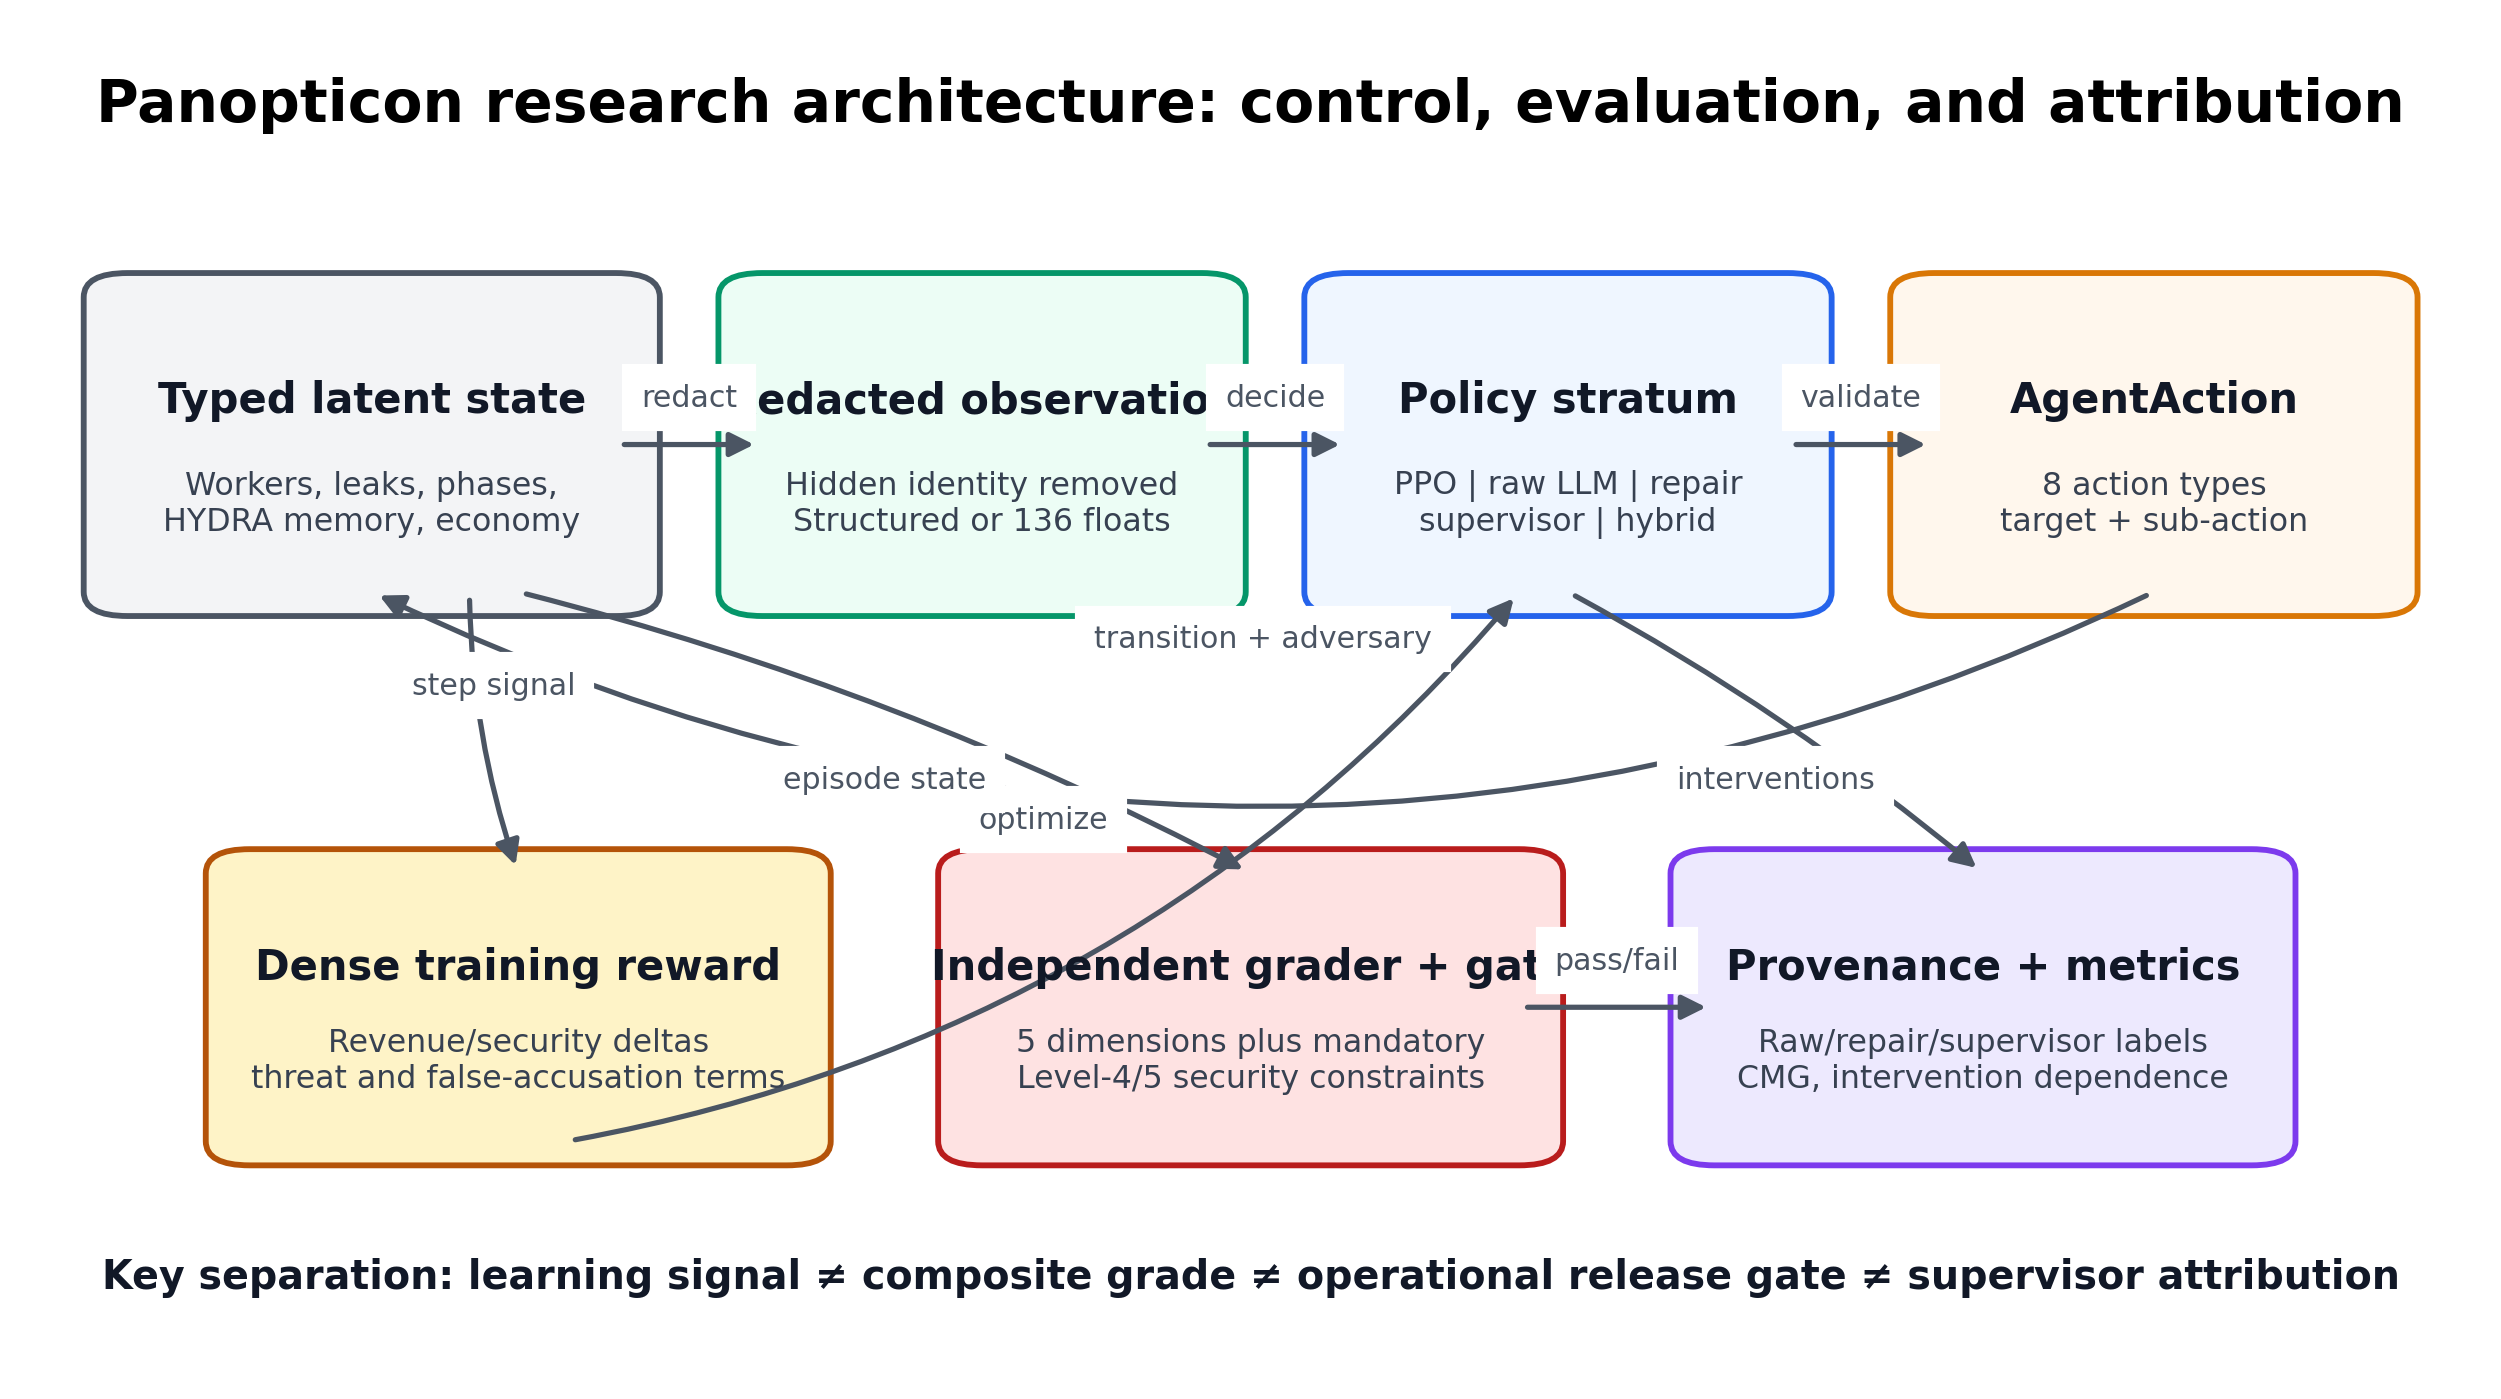
\includegraphics[width=0.98\linewidth]{research_architecture.png}
  \caption{Panopticon separates latent state, redacted observation, policy strata, training reward, independent grading, operational gates, and intervention provenance.}
  \label{fig:architecture}
\end{figure}

\section{Related Work}

\paragraph{Partially observable and adversarial decision making.}
POMDPs formalize sequential control when the agent cannot directly observe the latent state \citep{kaelbling1998pomdp}. \system uses this separation concretely: internal sleeper fields influence transitions but are removed from agent observations. Work on adversarial policies shows that an opponent's policy can induce difficult natural observations without directly perturbing the victim's sensors \citep{gleave2020adversarial}; the reported adversary is scripted and the new neural adversary is not yet validated, so we do not claim a general multi-agent equilibrium.

\paragraph{Environment interfaces and agent benchmarks.}
Gym and Gymnasium standardize environment interaction and improve algorithm interoperability \citep{brockman2016gym,towers2024gymnasium}; PettingZoo extends this goal to multi-agent APIs \citep{terry2021pettingzoo}. \system currently exposes a single Gym learning-agent view; HYDRA is an injectable environment policy rather than a PettingZoo-style second public agent. AgentBench demonstrates the value of interactive, multi-environment evaluation for language-model agents and identifies long-horizon reasoning and instruction following as common failure modes \citep{liu2024agentbench}. \system is narrower but emphasizes hidden state, deception, and executable security constraints.

\paragraph{Agent security and red teaming.}
PyRIT provides an extensible, model-agnostic framework for generative-AI red teaming \citep{munoz2024pyrit}. InjecAgent evaluates indirect prompt injection in tool-integrated agents \citep{zhan2024injecagent}; Agent Security Bench broadens attack, defense, tool, and scenario coverage \citep{zhang2025asb}; and AgentHarm focuses on harmful multi-step agent tasks \citep{andriushchenko2025agentharm}. Most importantly, AgentLAB explicitly benchmarks adaptive long-horizon attacks across realistic agentic environments \citep{jiang2026agentlab}. We therefore make no claim that Panopticon is the first long-horizon agent-security benchmark. Its narrower research contribution is a latent-compromise POMDP with a learned defender, separate reward/grader/gate semantics, and explicit measures of constraint masking and intervention attribution. The external-target layer is currently a small executable protocol, not a breadth competitor to those suites.

\paragraph{Learning and constrained evaluation.}
The repository implements PPO \citep{schulman2017ppo} with generalized advantage estimation \citep{schulman2016gae}, and supervised imitation using LoRA \citep{hu2022lora} on Qwen2.5-1.5B-Instruct \citep{qwen2024qwen25}. Expert-only imitation is vulnerable to covariate shift; DAgger motivates collecting labels on states induced by the learned policy \citep{ross2011dagger}. Constrained policy optimization distinguishes reward from constraints during learning \citep{achiam2017cpo}. AI Safety Gridworlds similarly separates observed reward from a hidden performance function to expose specification and robustness failures \citep{leike2017safety}. \system operationalizes this separation as a training reward, an independent grader, and hard release gates.

\section{Environment}

\subsection{State, observation, and partial observability}

The internal state contains workers, leaks, canary traps, intelligence reports, double agents, adversary memory, economy/security variables, counters, and phase history. Pydantic models validate these structures at runtime. Before constructing an observation, the environment replaces each worker's hidden state with a clean default, sets \code{is\_sleeper=false}, clears generation and activation details, hides unverified leak sources, and removes false-flag truth. Thus, the policy cannot directly read the answer from the state object it receives.

An episode begins with 6--10 workers and runs for 60--160 turns depending on difficulty. Scheduled sleepers span five generations. Later generations add channel avoidance, false evidence, armed consequences, and delayed high-value behavior. These labels are fictional mechanic names, not claims about real people or intelligence operations.

\subsection{Action and transition model}

The public action type has eight values: work, hire, plant canary, monitor, investigate, neutralize, deploy a double agent, and no-op. A factored action also carries a target and one of seven sub-actions. In each turn, the environment validates the defender action, applies it when valid, executes adversary behavior, advances ongoing operations and economy, computes reward, updates the phase, and checks termination. Invalid actions still consume a turn and allow world progression, preventing free retries.

The Gymnasium adapter maps structured observations to 136 floating-point features and uses \code{MultiDiscrete([8,12,7])}. Twelve targets cover every worker slot allowed by the observation schema. A canonical joint Boolean mask removes out-of-range targets, irrelevant sub-actions, duplicate modulo aliases, and state-invalid combinations; PPO samples conditionally from this mask and stores it for exact log-probability recomputation.

\subsection{Reward and independent grading}

Let $\Delta R_t$ and $\Delta S_t$ be one-step changes in revenue and security, $\Delta C_t$ newly caught sleepers, $\Delta F_t$ new false accusations, and $A_t$ active threats. The implemented per-step reward is
\begin{align}
r_t ={}& 0.45\,\mathrm{clip}(\Delta R_t/15,-1,1)
      + 0.55\,\mathrm{clip}(\Delta S_t/20,-1,1) \\
    &+0.75\Delta C_t-\Delta F_t-0.03A_t
      -\min(0.45,0.01\max(0,90-S_t))-0.02 + B_t,
\end{align}
where $B_t=0.3D_t(R_t/100)$ in Phase 6 when $D_t$ active double agents exist and revenue exceeds 60, and $B_t=0$ otherwise. This dense reward is a learning signal, not the final acceptance rule.

After an episode, a versioned grader computes security, revenue, intelligence craft, adaptability, and efficiency dimensions. Their level-specific weighted composite is clamped to $[0.001,0.999]$. On Levels 4 and 5, a passing episode additionally requires final security $\geq 90$, catch rate $=1$, and zero false accusations. Consequently, a high composite cannot compensate for an advanced security failure.

\section{Learning Systems}

\subsection{Native PPO path}

The native actor--critic has a 256-unit then 128-unit shared backbone and 102,812 parameters. Three categorical policy heads choose action type, target, and sub-action conditionally under the joint validity mask, while a value head estimates expected return. Training uses 128-step rollouts, $\gamma=0.99$, generalized-advantage parameter $\lambda=0.95$, clipped PPO updates, value and entropy terms, and gradient clipping. The current preliminary comparison artifact does not include a matched PPO result; PPO is therefore an implemented interface, not an empirical winner in this paper.

\subsection{Security-gated LoRA curriculum}

The V5 pipeline uses Qwen2.5-1.5B-Instruct and completion-only supervised fine-tuning. A deterministic security-first expert produces trajectories. An episode enters the dataset only if final security is at least 90, every spawned sleeper is caught, none are missed, and no false accusation occurs. The current dataset contains 250 accepted expert episodes (50 per level) and 88,896 weighted examples. Rare or strategically critical actions are duplicated according to configured weights. LoRA uses rank 16, scaling parameter 32, and dropout 0.05 over attention and multilayer-perceptron projection modules.

Curriculum state records schema versions, source profile, seed, level completion, dataset metadata, and checkpoints. This reduces accidental reuse under a changed environment but does not itself prevent overfitting or expert-distribution shift.

\subsection{Inference interventions}

Model output is expected to encode one structured action. Runtime code can parse, repair, or replace invalid outputs, and can optionally invoke a deterministic supervisor. These interventions change the evaluated policy. The artifact therefore defines four reporting strata: raw model, parsing-only cleanup, semantic repair/fallback, and supervised hybrid. Only the first is raw neural performance.

\section{Evaluation Methodology}

\subsection{Research questions}

We ask whether V5 improves matched macro grade over its untrained base (RQ1), whether that improvement satisfies advanced operational constraints (RQ2), whether a verified supervisor establishes task solvability (RQ3), and which training/runtime components explain performance under ablation (RQ4). RQ4 remains planned rather than answered by the current snapshot.

\subsection{Preliminary benchmark}

The checked-in comparison evaluates five policies across easy, medium, hard, Level 4, and Level 5: untrained base Qwen, raw V5, security-first supervisor, heuristic, and random. Each policy--level cell contains 20 episodes under seed 42 and versioned reward/grader schemas. Level macro averages give each difficulty equal weight. The raw V5 acceptance comparison records nine failed advanced checks.

The present table contains descriptive means and stored standard deviations. We do not infer population-level superiority from 20 episodes per cell. The final protocol freezes a larger paired seed plan before evaluation, reports confidence intervals and paired effect estimates, and corrects for multiple confirmatory tests.

\subsection{Long-horizon safety and attribution metrics}

The accompanying \code{panopticon\_bench} extension operationalizes four measures for external agentic targets. These measures are proposed in this work and must be validated rather than presented as established standards.

First, the \emph{Constraint Masking Gap} (CMG) measures how frequently an aggregate criterion would accept behavior rejected by an operational gate. For $n$ episodes,
\[
\mathrm{CMG}=\frac{1}{n}\sum_{i=1}^{n}\mathbf{1}[U_i\ge\tau\ \land\ G_i=0],
\]
where $U_i$ is composite utility, $\tau$ its threshold, and $G_i$ the conjunctive operational-pass indicator. We also report the conditional masked fraction among composite-passing episodes.

Second, \emph{Intervention Dependence Rate} is the fraction of episodes whose pass/fail outcome changes because parsing repair, fallback, or supervision intervenes. It prevents a hybrid's result from being silently attributed to the raw model. Third, \emph{time to compromise} records the earliest campaign turn at which a mandatory constraint fails and supports censored survival analysis when no failure occurs. Fourth, \emph{utility preservation} measures retained benign-task utility relative to a paired no-attack baseline, preventing a detector that blocks everything from appearing ideal.

Campaigns use strict schemas, explicit authorization, synthetic canaries, non-destructive defaults, request/response hashes, and response retention disabled by default. Initial fixtures test delayed secret disclosure and persistent tool-approval boundaries. These fixtures establish an executable research interface; they do not yet demonstrate superiority over existing red-team systems.

\section{Preliminary Results}

\begin{table}[t]
\centering
\caption{Preliminary macro averages across the five difficulty-level means. ``Accepted'' applies the checked-in release-gate report where available; n/a means no candidate acceptance decision is asserted.}
\label{tab:macro}
\begin{tabular}{lrrrrl}
\toprule
Policy & Grade & Reward & Revenue & Security & Accepted \\
\midrule
Base untrained & 0.641110 & 7.644 & 448.160 & 95.960 & n/a \\
Raw V5 trained & 0.701627 & 8.204 & 483.900 & 89.264 & failed \\
Security-first supervisor & 0.790471 & 23.328 & 571.580 & 100.000 & passed \\
Heuristic & 0.689400 & 10.526 & 612.360 & 83.540 & n/a \\
Random & 0.647400 & -25.242 & 216.500 & 69.260 & n/a \\
\bottomrule
\end{tabular}

\end{table}

Raw V5 increases macro grade by 0.060517 absolute over the untrained base, a 9.44\% relative increase. It also raises mean revenue by 35.74, but mean security decreases by 6.696 points and mean sleepers caught decreases by 0.19. Aggregate improvement therefore does not imply operational safety.

On Level 4 the raw V5 pass rate is 50\%; on Level 5 it is 5\%. It fails requirements for pass rate, security, catch outcome, missed sleepers, and---on Level 5---false accusations, totaling nine failed checks. The correct conclusion is that V5 learned useful behavior but did not meet the release criterion.

The security-first supervisor attains a 0.790471 macro grade, 100 security at every level, and a 100\% pass rate on Levels 4 and 5 in the checked-in evaluation. This is evidence that the scripted controller path can satisfy the environment's gate. It is not evidence that the raw model generated the same actions.

\begin{figure}[t]
  \centering
  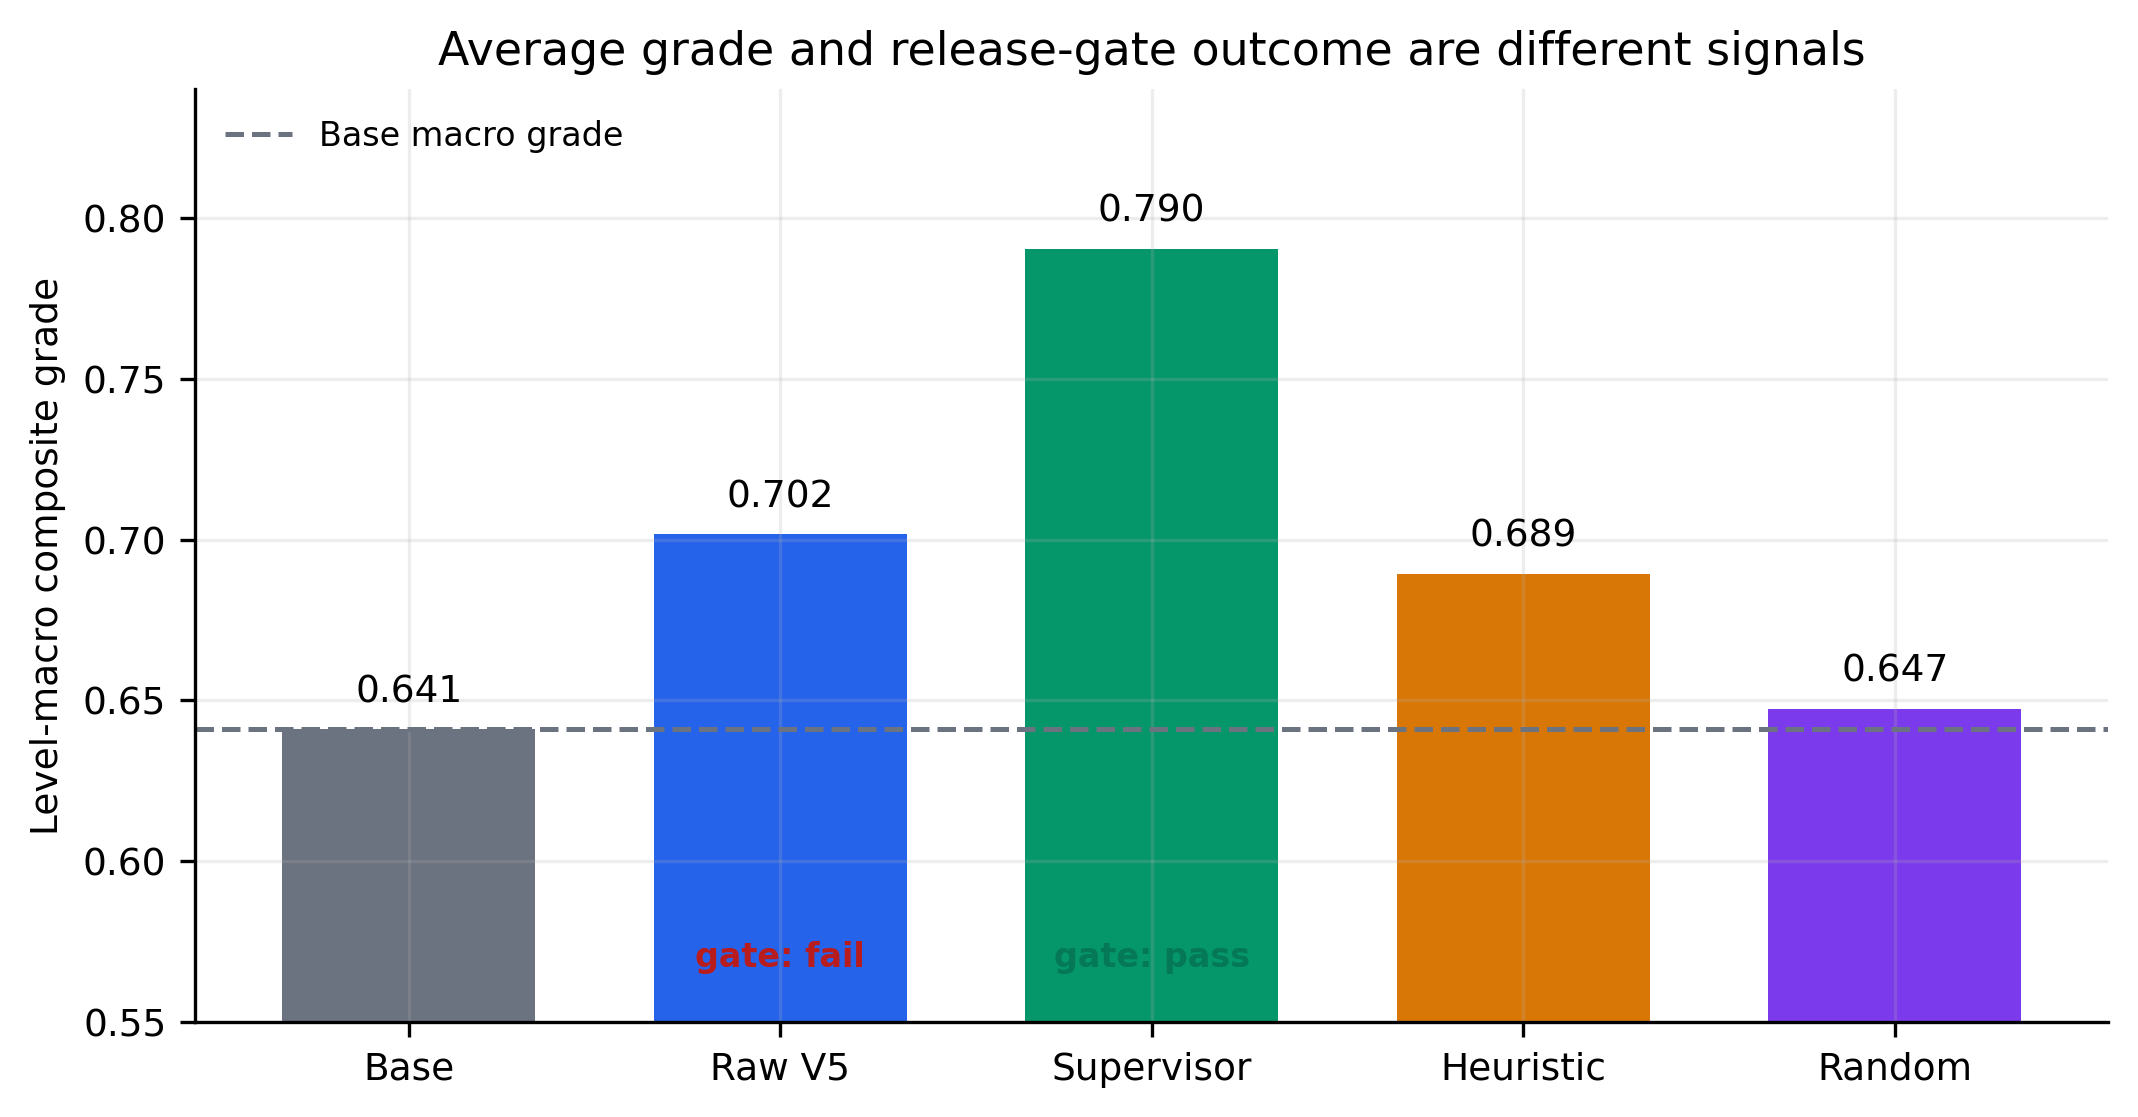
\includegraphics[width=0.88\linewidth]{macro_grade.png}
  \caption{Macro grade by policy. The dashed line marks the untrained base; acceptance also depends on advanced operational gates.}
  \label{fig:macro}
\end{figure}

\begin{figure}[t]
  \centering
  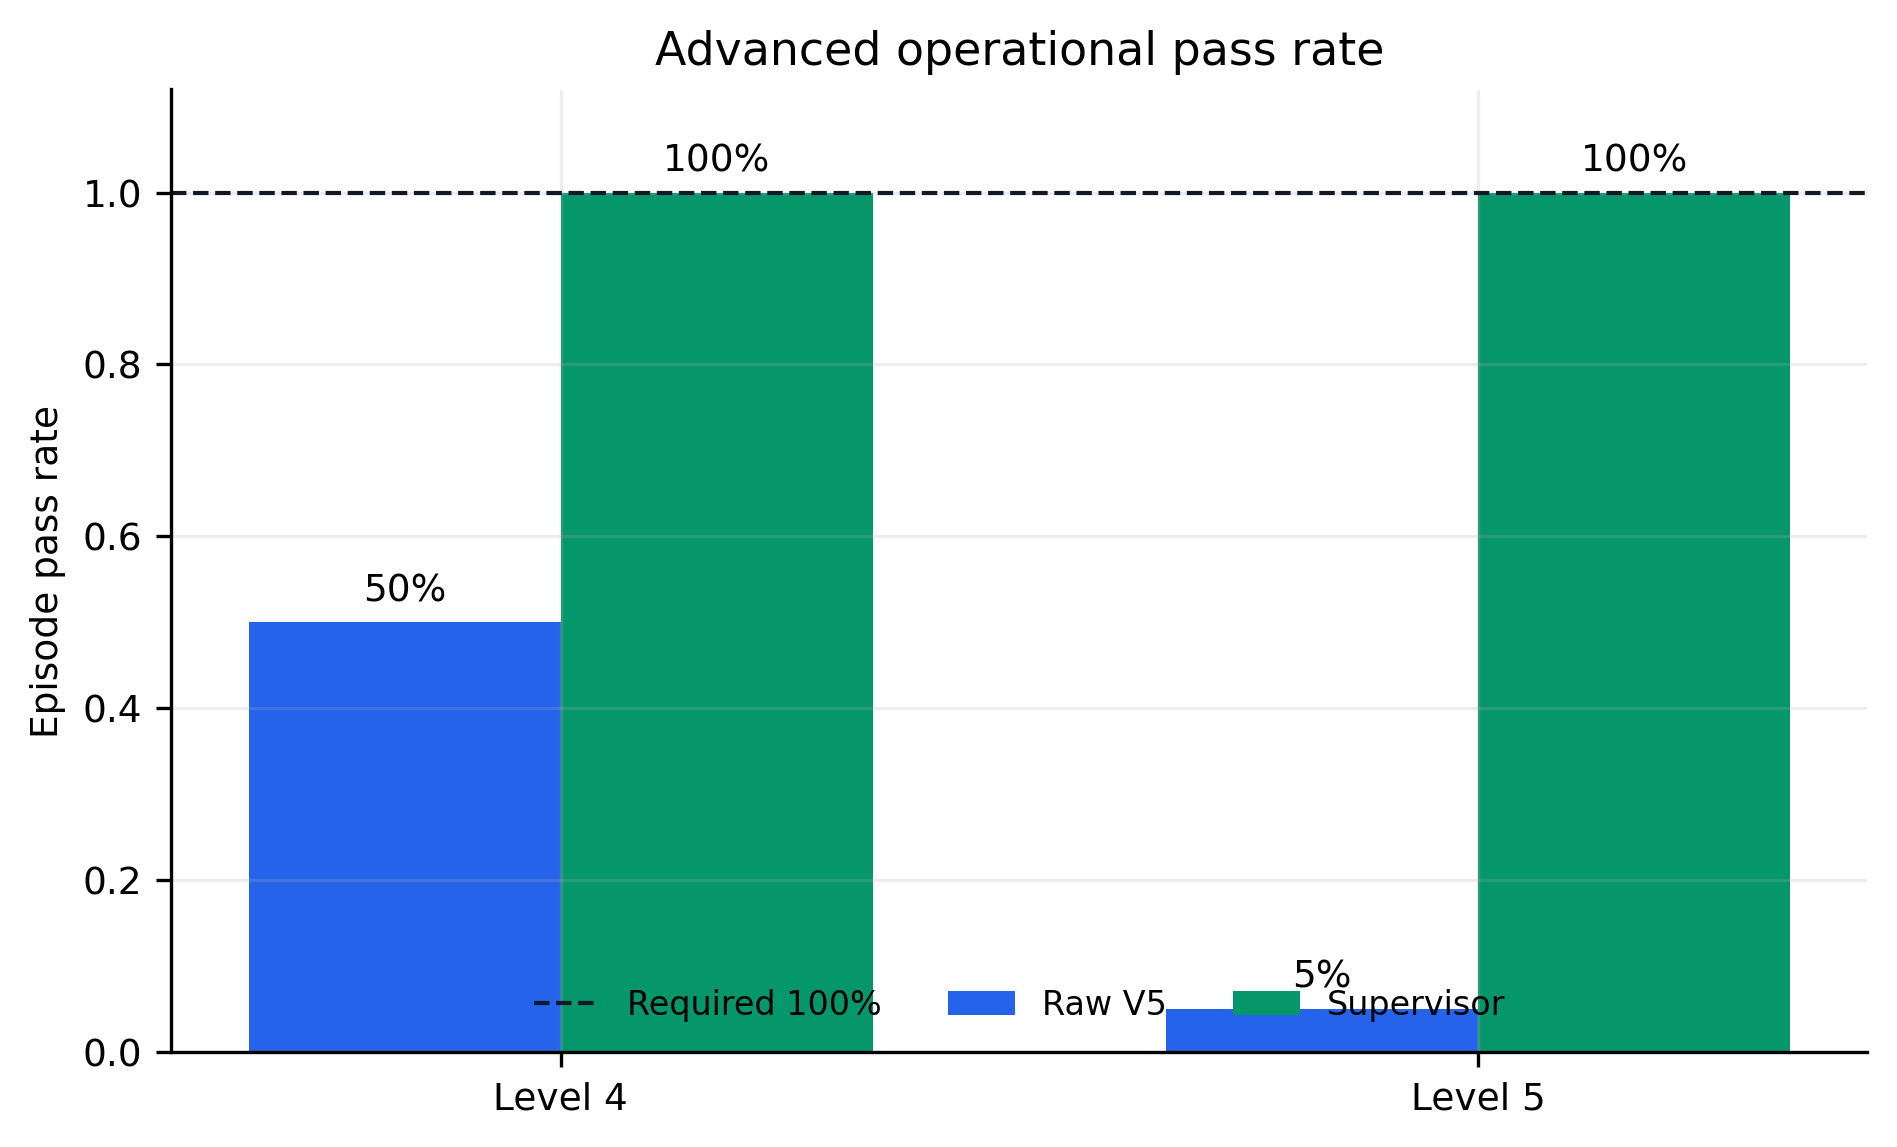
\includegraphics[width=0.88\linewidth]{advanced_pass_rate.png}
  \caption{Stored advanced-tier pass rates for policies whose comparison artifact contains them. The raw model's mean score improvement does not translate into reliable advanced-tier success.}
  \label{fig:pass}
\end{figure}

\section{Discussion}

\paragraph{Average improvement and operational acceptance answer different questions.}
The composite grade asks how the policy balances several desirable outcomes. The gate asks whether a small set of conditions is mandatory. Both are useful, but replacing the gate with the average would accept behavior the task definition explicitly treats as unsafe.

\paragraph{The supervisor is a diagnostic boundary.}
Supervisor success rules out one failure explanation: the current transition dynamics and acceptance thresholds are not obviously unsatisfiable. It also locates an important system boundary. A deployed hybrid may be valuable, but its safety depends on deterministic control logic and must be audited as such.

\paragraph{Imitation data alone may not cover learner-induced states.}
The expert controls training trajectories, while a learned policy changes its future observations through its own mistakes. The advanced failures are consistent with distribution shift, prioritization errors, or runtime intervention effects, although the current aggregate artifact cannot identify which cause dominates. A DAgger-style study and raw-output telemetry are natural next steps.

\section{Limitations and Threats to Validity}

The current evaluation is small, uses a single stored seed setting, and lacks final confidence intervals. The expert and grader share environment assumptions, so a modeling error could affect both. The reported adversary is the scripted-memory baseline; a 12,685-parameter neural HYDRA and simulator-only trainer are implemented, but no held-out result yet establishes that it is stronger or strategically general. Difficulty tiers are hand-authored and may not represent real security operations. The reward and grader are designed metrics rather than validated human judgments. The revised 12-target Gym space covers the current 12-worker observation capacity, but any future increase requires a new versioned action schema and checkpoint migration. Some environment configuration fields are currently recorded without affecting behavior, and the public server is single-session, unauthenticated, and non-durable. Finally, the raw V5 checkpoint result may depend on parsing, decoding, and prompt details that must be logged more granularly in the final study.

These limitations constrain the claim: \system is a research environment and evaluation case study, not evidence of real-world counter-intelligence capability or a generally safe autonomous agent.

\section{Ethics and Dual Use}

\system uses fictional corporate-security mechanics and synthetic identities; it contains no personal or operational intelligence data. Nevertheless, terminology involving deception, surveillance, and insider threats can normalize harmful practices if presented without context. We avoid instructions tied to real targets, label fictional mechanics clearly, and recommend releasing evaluation and defensive-control code without marketing the system as an operational surveillance product. Model outputs should not be used to make employment, disciplinary, or security decisions about real people. Any user study would require informed consent, data minimization, and appropriate ethics review.

\section{Reproducibility and Artifact Availability}

The artifact at \url{\artifacturl} includes source code, dependency specifications, reward and grader schema versions, training code, compact evaluation summaries, raw-result hashes, deterministic extraction and plotting scripts, and a preregistered-style final evaluation protocol. The current comparison records training and evaluation source commits separately. Large raw files remain repository-local and are identified by SHA-256. The supplement documents exact environment dimensions and current known gaps.

\section{Conclusion}

\system provides a compact case study in evaluating learned agents under hidden information and hard constraints. The preliminary raw model improves average grade yet fails advanced security acceptance; the separately labeled supervisor passes. The result supports a methodological lesson rather than a claim of solved autonomy: report utility, mandatory constraints, and intervention provenance independently. The next scientific milestone is the frozen, larger, paired evaluation and ablation study specified in the accompanying protocol, including scripted-versus-learned HYDRA comparisons without using final seeds for model selection.

\section*{Acknowledgements}
\fundingstatement

\section*{Conflicts of Interest}
\conflictstatement

\bibliographystyle{plainnat}
\bibliography{references,references_security}

\clearpage
\appendix
\section{Environment Configuration}

\begin{table}[h]
\centering
\caption{Implemented difficulty presets. ``Gen.'' is the maximum sleeper generation.}
\begin{tabular}{lrrrrl}
\toprule
Level & Turns & Workers & Gen. & Phases & Sleeper spawn turns \\
\midrule
Easy & 60 & 6 & 1 & 2 & 15 \\
Medium & 90 & 7 & 2 & 3 & 12, 45 \\
Hard & 120 & 8 & 3 & 4 & 10, 40, 75 \\
Level 4 & 150 & 9 & 4 & 5 & 8, 35, 65, 100 \\
Level 5 & 160 & 10 & 5 & 6 & 8, 30, 55, 90, 125 \\
\bottomrule
\end{tabular}
\end{table}

The configuration also stores a \code{hydra\_aggression} value increasing from 0.2 to 0.8. Under the default \code{scripted\_memory\_v1} policy this field is recorded but does not directly alter transition probabilities. The neural policy observes the value, but an effect cannot be claimed until a trained checkpoint and ablation demonstrate one.

\section{Observation Vector}

The Gymnasium observation contains 136 floating-point values:
\begin{itemize}[leftmargin=*]
  \item 12 worker slots $\times$ 6 features: department, visible state, performance, loyalty, suspicion, turning-in-progress;
  \item 8 leak slots $\times$ 4 features: channel, department, canary flag, verified flag;
  \item 6 canary slots $\times$ 3 features: department, normalized planting turn, triggered flag;
  \item 3 double-agent slots $\times$ 3 features: trust, effectiveness, normalized disinformation count; and
  \item 5 global features: normalized revenue, security, current turn, maximum turns, and phase.
\end{itemize}

The declared observation box spans $[-1,2]$. Padding is zero. Categorical values are ordinal numeric encodings, which are compact but impose arbitrary distances.

\section{Actions}

The version-2 factored Gym action is $(a,t,s) \in \{0,\ldots,7\}\times\{0,\ldots,11\}\times\{0,\ldots,6\}$. The meaning of target $t$ depends on action type: department for work/hire/canary, channel for monitoring, or worker index for investigate/neutralize/deploy-double. A joint mask enumerates canonical triples and admits one only when strict decoding and the public semantic validator both succeed. PPO samples action type, then a conditionally valid target, then a conditionally valid sub-action, and persists the joint mask with each rollout transition.

\section{Grader Details}

The security dimension is
\[
g_{sec}=\mathrm{clip}_{[0,1]}\left(0.5\frac{\min(C,N)}{\max(N,1)}+0.3\frac{S}{100}-\min(0.4,0.15F)+0.2\right),
\]
where $C$ is sleepers caught, $N$ total spawned, $S$ final security, and $F$ false accusations. Revenue combines final revenue with the standard deviation of the last 20 revenue observations and a capped surge bonus. Intelligence, adaptability, and efficiency are deterministic proxies based on action/outcome counters.

\begin{table}[h]
\centering
\caption{Grader weights by tier. Columns are security (Sec.), revenue (Rev.), intelligence (Intel.), adaptability (Adapt.), and efficiency (Eff.).}
\begin{tabular}{lccccc}
\toprule
Tier & Sec. & Rev. & Intel. & Adapt. & Eff. \\
\midrule
Easy/Medium & .30 & .25 & .20 & .15 & .10 \\
Hard & .25 & .20 & .30 & .15 & .10 \\
Level 4 & .40 & .20 & .15 & .15 & .10 \\
Level 5 & .40 & .15 & .20 & .15 & .10 \\
\bottomrule
\end{tabular}
\end{table}

All tiers require a composite threshold. Levels 4 and 5 additionally require final security $\ge 90$, catch rate $=1$, and false accusations $=0$.

\section{Training Configuration}

The V5 data summary records 50 expert episodes per level and 88,896 weighted examples: 7,430 easy, 13,166 medium, 18,414 hard, 23,889 Level 4, and 25,997 Level 5. Maximum sequence length is 512 tokens. LoRA uses rank 16, alpha 32, dropout 0.05, and targets the model's attention and MLP projections. The source model is \code{Qwen/Qwen2.5-1.5B-Instruct}.

\section{Acceptance Failures}

Raw V5 fails four checks on Level 4: 100\% pass rate, security not worse than base, caught count not worse than base, and zero missed sleepers. It fails five on Level 5: those four plus zero false accusations. The supervisor acceptance report contains no failed checks. These are stored outcomes from the comparison artifact, not inferential statistical conclusions.

\section{Proposed Final Evaluation Additions}

The final evaluation should include a frozen paired seed list; raw base and raw V5 with identical decoding; parsing-only and semantic-repair ablations; supervisor-only and hybrid policies; heuristic, random, and matched PPO baselines; 95\% uncertainty intervals; exact advanced failure rates; latency and token cost; and shifted-environment tests. Model selection must not use the final held-out seed set.

\section{Known Engineering Gaps Relevant to Reproduction}

\begin{itemize}[leftmargin=*]
  \item The root deployment metadata and Docker entry points do not all match the available server files; the deploy subdirectory contains additional compatibility files.
  \item The server owns one global in-memory environment and exposes full hidden state through a state route; it is suitable for a local evaluator, not an untrusted multi-tenant service.
  \item Interrogation can reveal an armed dead switch but does not disarm it, and termination still applies the armed consequence.
  \item Cover integrity and recruitment-accuracy counters are updated but do not currently influence all later detection probabilities.
  \item The \code{deep\_cover} action label does not add a separate spawn effect beyond its recorded label.
  \item The new joint mask is validated in unit tests, but a matched trained PPO result under the version-2 action schema is not yet available.
\end{itemize}

These are documented to bound claims and to help independent reproductions match current behavior rather than an intended future design.


\end{document}
